\documentclass{article}
\usepackage[T1]{fontenc}
\usepackage{lmodern}
\usepackage{graphicx}
\usepackage{amsmath,amssymb}
\usepackage[a4paper,margin=2cm]{geometry}
\usepackage[absolute,overlay]{textpos}
\setlength{\TPHorizModule}{1mm}
\setlength{\TPVertModule}{1mm}
\usepackage[indonesian]{babel}
\usepackage{hyperref}
\setlength{\emergencystretch}{2em}
% unit: Halaman 16

\begin{document}

% === Halaman 16 (llm) ===

\section*{Renaissance Steganography}

\vspace{10mm}

Tahun 1499, Johannes Trithemius menulis buku \textbf{Steganographia}, yang menceritakan tentang metode steganografi berbasis karakter

\vspace{10mm}

Johannes Trithemius \\ (1404--1472 )

\vspace{10mm}

Selanjutnya tahun 1518 dia menulis buku tentang steganografi dan kriptografi, berjudul \textbf{Polygraphiae}.

% deskripsi: Potret Johannes Trithemius
% bbox normalisasi: [0.0700, 0.0900, 0.2500, 0.4400]
\begin{textblock*}{37.80mm}(14.70mm,26.73mm)
\noindent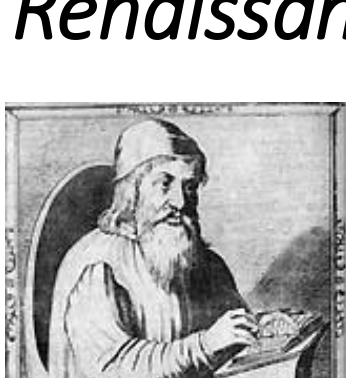
\includegraphics[width=37.80mm,height=103.95mm]{../../images/llm/page_016_img_01.png}%
\end{textblock*}

% deskripsi: Halaman judul buku Steganographia
% bbox normalisasi: [0.2800, 0.2000, 0.6400, 0.7700]
\begin{textblock*}{75.60mm}(58.80mm,59.40mm)
\noindent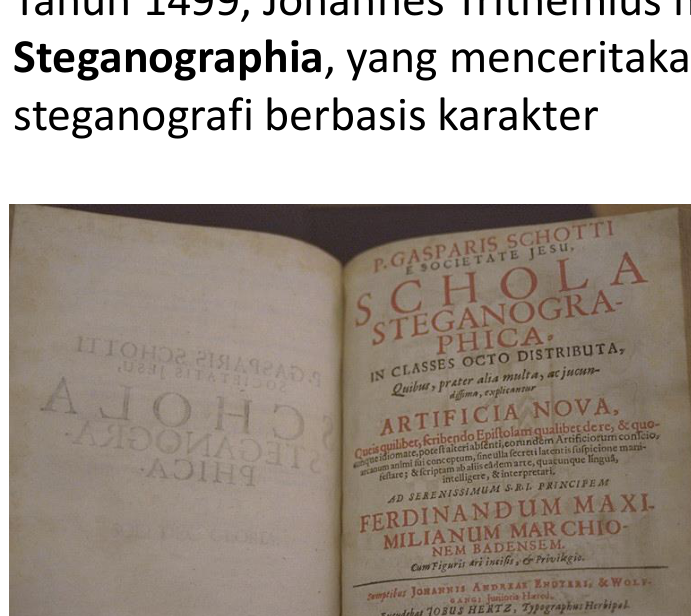
\includegraphics[width=75.60mm,height=169.29mm]{../../images/llm/page_016_img_02.png}%
\end{textblock*}

% deskripsi: Halaman judul buku Polygraphiae
% bbox normalisasi: [0.6900, 0.2000, 0.8700, 0.6500]
\begin{textblock*}{37.80mm}(144.90mm,59.40mm)
\noindent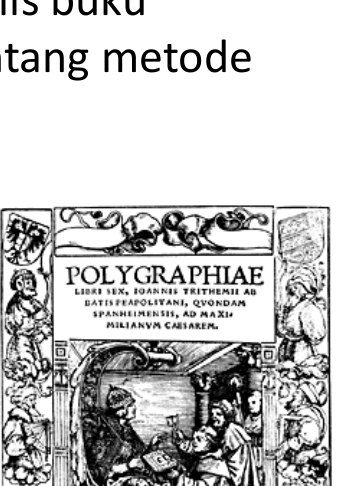
\includegraphics[width=37.80mm,height=133.65mm]{../../images/llm/page_016_img_03.png}%
\end{textblock*}

\end{document}
